\documentclass{beamer}
\usetheme{Warsaw}

\usepackage{graphicx} % Allows including images
\usepackage{booktabs} % Allows the use of \toprule, \midrule and \bottomrule in tables
\usepackage{listings}
\usepackage[utf8]{inputenc}
\usepackage[overlay,absolute]{textpos}
\usepackage[]{algorithm2e}
\usepackage{amssymb}
\usepackage{tikz}
\usetikzlibrary{arrows, automata}

\AtBeginSection[]
{
\begin{frame}<beamer>
\frametitle{Plan}
\footnotesize{
\tableofcontents[
  currentsection,
  hideothersubsections
]
}
\end{frame}
}

\lstset{language=C++,
                basicstyle=\ttfamily,
                keywordstyle=\color{green}\ttfamily,
                stringstyle=\color{red}\ttfamily,
                commentstyle=\color{cyan}\ttfamily,
                morecomment=[l][\color{magenta}]{\#}
}

\setbeamercolor{normal text}{fg=white,bg=black!90}
\setbeamercolor{structure}{fg=white}

\setbeamercolor{alerted text}{fg=red!85!black}

\setbeamercolor{item projected}{use=item,fg=black,bg=item.fg!35}

\setbeamercolor*{palette primary}{use=structure,fg=structure.fg}
\setbeamercolor*{palette secondary}{use=structure,fg=structure.fg!95!black}
\setbeamercolor*{palette tertiary}{use=structure,fg=structure.fg!90!black}
\setbeamercolor*{palette quaternary}{use=structure,fg=structure.fg!95!black,bg=black!80}

\setbeamercolor*{framesubtitle}{fg=white}

\setbeamercolor*{block title}{parent=structure,bg=black!60}
\setbeamercolor*{block body}{fg=black,bg=black!10}
\setbeamercolor*{block title alerted}{parent=alerted text,bg=black!15}
\setbeamercolor*{block title example}{parent=example text,bg=black!15}

\author[Félix-Antoine Ouellet]{Félix-Antoine Ouellet}

\title[PolyOpt\hspace{2em}\insertframenumber/\inserttotalframenumber]{Compilation polyhédrale}

\institute{Université de Sherbrooke}

\date{4 décembre 2014}

\begin{document}

\begin{frame}
\titlepage % Print the title page as the first slide
\end{frame}

\begin{frame}
\tableofcontents[hideallsubsections]
\end{frame}

\section{Motivation}
\begin{frame}
\frametitle{L'ère du parallélisme}

\end{frame}

\begin{frame}
\frametitle{Problèmes courants}
\framesubtitle{Optimisations des boucles}
Les compilateurs modernes sont très loin derrière la théorie
\begin{itemize}
\item Fusion
\item Tuilage
\item \textit{Skewing}
\item Etc...
\end{itemize}
\end{frame}

\begin{frame}
\frametitle{Problèmes courants}
\framesubtitle{Parallélisation d'applications existantes}
Comment améliorer la performance de \textit{legacy code}?
\begin{itemize}
\item Mettre tout à terre et recommencer
\item Payer des développeurs pour améliorer des sections critiques
\item Espérer qu'un outil améliore magiquement la situation
\end{itemize}
\end{frame}

\begin{frame}
\frametitle{Problèmes courants}
\framesubtitle{Rendre le parallélisme accessible}
On cherche toujours les meilleures abstractions pour le calcul parallèle
\begin{itemize}
\item \textit{Threads}
\item Tâches
\end{itemize}
\end{frame}

\section{Compilation traditionnelle}
\subsection{Bases de la compilation}
\begin{frame}
\frametitle{Notions importantes}
\begin{itemize}
\item Transforme un programme écrit dans un langage (de haut niveau) en un programme écrit dans un autre langage (de bas niveau).
\item Maintient la sémantique du programme original.
\end{itemize}
\end{frame}

\begin{frame}
\frametitle{Architecture usuelle}
\begin{center}
\begin{tikzpicture}[-,>=stealth',shorten >=1pt,auto,node distance=4.5cm,
  thick,main node/.style={rectangle,draw,font=\sffamily\Large\bfseries}]

  \draw[white] (0, 0) rectangle (2, 3);
  \draw[white] (2, 0) rectangle (4, 3);
  \draw[white] (4, 0) rectangle (6, 3);
  
  \node[draw=none] (1) at (1, 1.5) {\textit{Frontend}};
  \node[draw=none] (2) at (3, 1.5) {\textit{Optimizer}};
  \node[draw=none] (3) at (5, 1.5) {\textit{Backend}};
  \node[draw=none] (4) at (-1.5, 1.5) {Code source};
  \node[draw=none] (5) at (7.5, 1.5) {Code machine};
  
\end{tikzpicture}
\end{center}
\begin{textblock}{6}(4, 9.65)
	$\rightarrow$
\end{textblock}
\begin{textblock}{6}(12, 9.65)
	$\rightarrow$
\end{textblock}
\end{frame}

\subsection{Processus de compilation}
\begin{frame}[fragile]
\frametitle{Étape 1 - AST}
\begin{columns}
    \begin{column}{0.5\textwidth}
    \footnotesize{
\begin{lstlisting}
int countOdd(int A[],
             int N) {
  int cpt = 0;

  for (int i = 0; i < N; 
       ++i)
    if (A[i] % 2 == 1)
      cpt++;

  return cpt;
}
\end{lstlisting}}
    \end{column}
    \begin{column}{0.5\textwidth}
\colorbox{white}{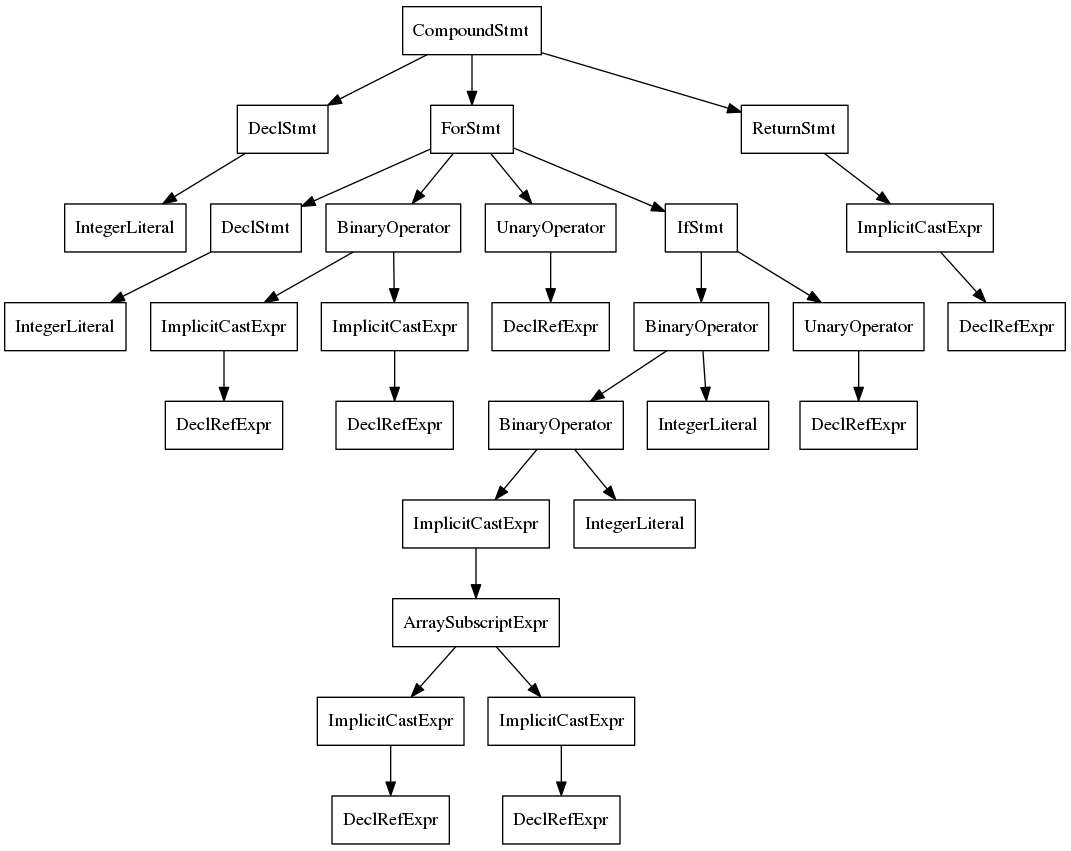
\includegraphics[scale=0.15]{AST.png}}
    \end{column}
\end{columns}
\begin{textblock}{6}(7.1, 9)
	\Huge{$\Rightarrow$}
\end{textblock}
\end{frame}

\begin{frame}
\frametitle{Étape 2 - CFG}
\begin{columns}
    \begin{column}{0.5\textwidth}
\colorbox{white}{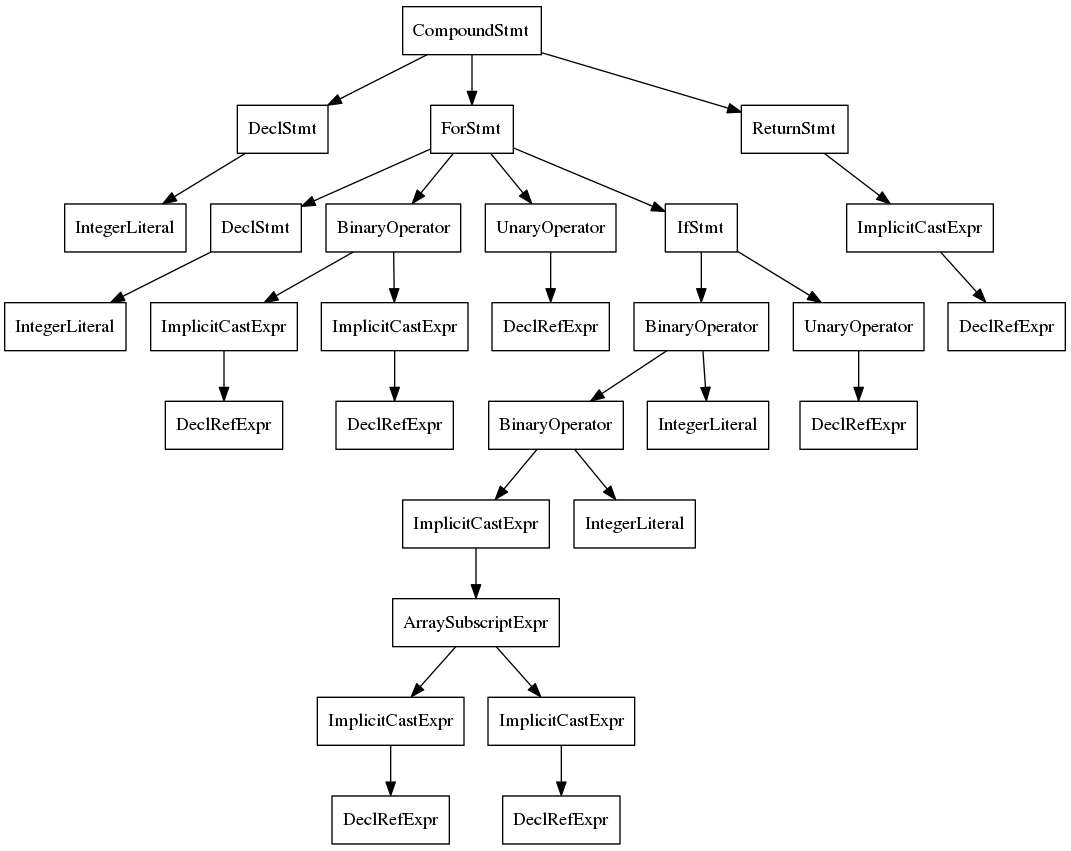
\includegraphics[scale=0.15]{AST.png}}
    \end{column}
    \begin{column}{0.5\textwidth}
\begin{center}
\colorbox{white}{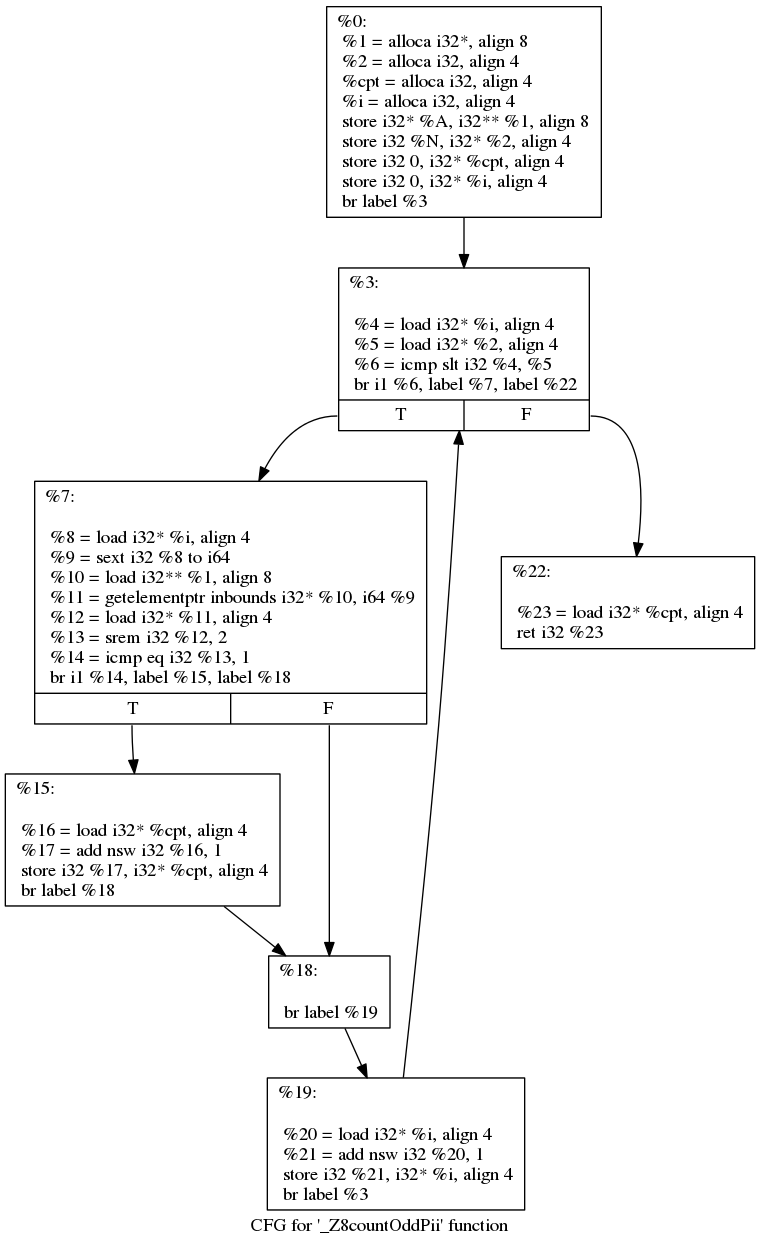
\includegraphics[scale=0.13]{cfg.png}}
\end{center}
    \end{column}
\end{columns}
\begin{textblock}{6}(8.35, 9)
	\Huge{$\Rightarrow$}
\end{textblock}
\end{frame}

\begin{frame}
\frametitle{Représentation intermédiaire}
\framesubtitle{Illustration}
\begin{center}
\colorbox{white}{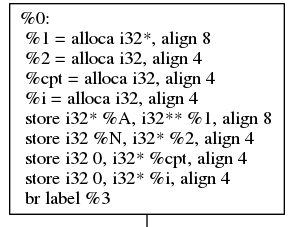
\includegraphics[scale=0.7]{basic block.png}}
\end{center}
\end{frame}

\begin{frame}
\frametitle{Représentation intermédiaire}
\framesubtitle{Raisonnement}
\begin{itemize}
\item Mieux analyser le programme donné
\item Permettre des optimisations indépendantes de la machine
\item Vérifier les optimisations effectuées
\end{itemize}
\end{frame}

\section{Analyse de dépendences}
\begin{frame}
\frametitle{Définition}
Situation dans laquelle deux instructions accèdent à la même donnée.
\end{frame}

\begin{frame}[fragile]
\frametitle{Importance des dépendences}
Indique quelles transformations sont légales \\
\begin{lstlisting}
for (int i = 0; i < N; ++i)
  for (int j = 0; j < N; ++j)
    A[i][j] = A[i+1][j-1];
\end{lstlisting}
\begin{textblock}{6}(11, 8)
	\begin{itemize}
	\item[\checkmark] Déroulement
	\item[$\times$] Inter-échange
	\end{itemize}
\end{textblock}
\end{frame}

\begin{frame}[fragile]
\frametitle{Importance des dépendences}
Indique les opportunités de parallélisme \\
\begin{lstlisting}
for (int i = 0; i < N; ++i)
  for (int j = 0; j < N; ++j)
    A[i][j] = A[i+1][j-1];

\end{lstlisting}
\begin{itemize}
\item Parallélisme d'intructions au niveau de la boucle interne
\item Parallélisme de fils d'exécution au niveau de la boucle externe
\end{itemize}
\end{frame}

\begin{frame}
\frametitle{Représentation}
\framesubtitle{Vecteur de distance}
Vecteur \textbf{d(i, j)} tel que \textbf{d(i, j)$_{k}$} = \textbf{j}$_{k}$ - \textbf{i}$_{k}$ où \textbf{i} et \textbf{j} sont des vecteurs d'itérations.
\end{frame}

\begin{frame}[fragile]
\frametitle{Représentation}
\framesubtitle{Vecteur de distance}
\begin{lstlisting}
for (int i = 0; i < N; ++i)
  for (int j = 0; j < M; ++j)
    for (int k = 0; k < L; ++k)
      A[i+1][j][k-1] = A[i][j][k] + 10;
    
\end{lstlisting}

\textbf{d(i, j)$_{k} = (-1, 0, 1)$}
\end{frame}

\begin{frame}
\frametitle{Représentation}
\framesubtitle{Vecteur de direction}
Vecteur \textbf{D(i, j)} tel que: 
\[ D(i, j)_{k} = \left\{
  \begin{array}{l l}
    "<" & \quad \text{si $d(i, j)_{k} > 0$}\\
    "=" & \quad \text{si $d(i, j)_{k} = 0$}\\
    ">" & \quad \text{si $d(i, j)_{k} < 0$}
  \end{array} \right.\]
\end{frame}

\begin{frame}[fragile]
\frametitle{Représentation}
\framesubtitle{Vecteur de direction}
\begin{lstlisting}
for (int i = 0; i < N; ++i)
  for (int j = 0; j < M; ++j)
    for (int k = 0; k < L; ++k)
      A[i+1][j][k-1] = A[i][j][k] + 10;
    
\end{lstlisting}

\textbf{D(i, j)$_{k} = (<, =, >)$}
\end{frame}

\begin{frame}
\frametitle{Tests de dépendences}

\end{frame}

\begin{frame}
\frametitle{Points à améliorer}
Ce modèle éprouve de la difficulté au niveau de:
\begin{itemize}
\item Parallélisme de niveau plus haut niveau que celui des instructions
\item Parallélisme de tâches
\item Distribution de données
\end{itemize}
\end{frame}

\section{Approche polyhédrale}
\subsection{Représentation}
\begin{frame}
\frametitle{Représentation}

\end{frame}

\subsection{Optimisations}

\subsection{Limitations}
\begin{frame}
\frametitle{Limitations}
\begin{itemize}
\item Accès non affines
\item Boucles irrégulières
\end{itemize}
\end{frame}

\section{Parallélisation automatique}
\begin{frame}
\frametitle{Intuition}

\end{frame}

\subsection{Mémoire partagée}
\begin{frame}
\frametitle{Mémoire partagée}

\end{frame}

\subsection{Mémoire distribuée}
\begin{frame}
\frametitle{Mémoire distribuée}

\end{frame}

\subsection{Support présent}
\begin{frame}
\frametitle{Support présent}
\begin{itemize}
\item GCC (Graphite)
\item LLVM (Polly)
\item Langages expérimentaux (X10)
\item Plateformes expérimentales (PLUTO)
\end{itemize}
\end{frame}

\section{Conclusion}
\begin{frame}
\frametitle{Conclusion}
\begin{itemize}
\item Offre une façon différente de raisonner sur l'optimisation de boucles et la parallélisation automatique
\item Représente possiblement la meilleure chance de produire du parallélisme implicite
\end{itemize}
\end{frame}

\end{document}